% -%-%-%-%-%-%-%-%-%-%-%-%-%-%-%-%-%-%-%-%-%-%-%-%-%
% PIM380                                           % 
% Data:28/06/2013                                  %
% Paris,France                                     % 
% Groupe:                                          %
% - Tiago Chedraoui Silva                          %  
% - Vinicius Dias Gardelli                         %
% -%-%-%-%-%-%-%-%-%-%-%-%-%-%-%-%-%-%-%-%-%-%-%-%-%

\documentclass[a4paper,12pt]{article}

\usepackage[francais,listings,algo]{pim}
\bibliographystyle{apalike}  

% Cover %
\def \ttprofname{Prof \textordmasculine.~Dr \textordmasculine.Tamy Boubekeur} % teachers name
\def \ttabrv{PIM380 } % abbreviation of names class
\def \ttabrvxt{} % period
\def \mytitle{Reconstruction 3D temps-réel HD de visages} % Big title
\def \ttauthi{Tiago~Chedraoui~Silva} % author's name
\def \ttxti{Casier: 361 } % Extra text right side of name
\def \ttauthii{Vinicius~Dias~Gardelli} % author's name
\def \ttxtii{Casier: 379 } % Extra text right side of name
\def \ttdate{Juillet 25, 2013} % date

%\spc{1.5}
\begin{document}
\thispagestyle{empty}
\titleTMB 
 % \begin{titlepage}
 % \thispagestyle{empty}
 % \begin{center}  \begin{figure}[h!]
 %   \begin{center}
 %     
\includegraphics[scale=0.1]{img/logo.jpg}
 %   \end{center}
 % \end{figure}
 %\end{center}
 % %\vspace{0.3cm}
 % \begin{center} 
 %   {\Large \textsc{Reconstruction 3D temps-réel HD de visages}} 
 %   \\\vspace{0.5cm}
 %   {\textsl{Rapport Projet PIM - Projet d’Innovation Master}}
 %   \\\vspace{1cm}
 %   \begin{tabular}{rl}
 %     \textbf{Elève}:       & \ttauthi \\
 %     \textbf{Elève}:       & \ttauthi \\
 %     \textbf{Professeur}: & \ttprofname
 %   \end{tabular}
 %   % Instituto de computação\\
 %   \vspace{0.5cm}
 %   \\ \ttdate     
 % \end{center}
 % \vspace{0.5cm}
%  \begin{abstract}
%    Dans les deux décennies, les animations faciales ont eu plusieurs aproches. Actuellment, les dernières méthodes sont basée sur une capture passive dont la configuration est presque entièrement automatiques. 
%    Le but de ce projet est de réproduire une reconstruction 3D de visages à travers d'une méthode de capture passive qui utilisera que des outils périphériques peu coûteux, qui sont plus accessibles à la majorité des personnes.
 % \end{abstract}
  % Sumário
%\tableofcontents

%\end{titlepage} 

\newpage
\thispagestyle{empty}
\begin{abstract}

Dans les deux décennies, les animations faciales ont eu plusieurs approches.
Actuellment, les dernières méthodes sont basées sur une capture
passive dont la configuration est presque entièrement automatiques. 

Le but de ce projet est de reproduire une reconstruction 3D de visages
à travers une méthode de capture passive qui utilisera que des outils
périphériques peu coûteux, qui sont plus accessibles à la majorité des
personnes. 

\end{abstract}

\newpage
\thispagestyle{empty}
\tableofcontents
\newpage
\setcounter{page}{1}

\section{Introduction}

Les animations faciales ont eu plusieurs approches dans les deux
décennies, comme par exemple l'utilisation d'éclairage active et
l'utilisation des marqueurs. Actuellement, les dernières recherches,
ont convergé aux captures passives dont la configuration est presque
entièrement automatiques, ce qui diminuera le temps de préparation
nécessaire pour que la capture soit possible, ainsi comme sera moins invasive aux
acteurs.

Cependant, malgré des avancées majeures dans ce type de capture, une
technique pour capturer des performances expressives très détaillées
qui évite détérioration avec le temps doit encore être réalisée.

Le but de ce projet est de produire une reconstruction 3D d'une
surface dynamique de visages à travers une méthode de capture passive
qui utilisera des outils périphériques peu coûteuses, par conséquent
en étant plus accessibles à la majorité des personnes, comme par
exemple une Kinect.

% L'objectif du projet est la recherche et la mise au point d'un
% algorithme de reconstruction 3D de surface dynamique appliqué
% spécifiquement à un visage. 

%Les données d'entrées sont provienues d'une kinects.

\section{Etat de l'art}

Les animations faciales a eu plusieurs approches dans les deux décennies, 
parmi eux: l'utilisation des modèles de visage qui sont ajustées aux images, 
l'utilisation de l'éclairage actif et utilisation des marqueurs.

En vue d'avoir une méthode moins coûteux et moins intrusif, les dernières
méthodes sur les animations faciales sont basée sur des captures passives.

% dont la configuration est presque entièrement automatiques.   [Bradley et al. 2010; Popa et al. 2010]. 

Dans cette section, nous aurons une bref description de chaque
approche.

\subsection*{Ajuster les faces aux images}
Une approche pour la capture des faces est commencer avec un modèle
de visage déformable, puis de déterminer les paramètres qui
correspondent le mieux au modèle des images ou des vidéos d'un acteur
performant. 

Un inconvenient de cette approche est qu'il exige un grande nombre de
calculs et pour qu'il soit traitable, le modèle de visage doit être
d'une faible résolution.

Ainsi, comme résultat, il n'est généralement pas possible d'obtenir les
détails les plus fins, qui sont responsables pour les expressions et
réalisme de la scène.

De plus, le visage déformable a tendance à être très générique, de
sorte que les animations résultant de ce genre de téchnique souvent ne
ressemblent pas à l'acteur capturé.

\subsection*{Marqueurs et éclairage actif}

Une autre approche commune pour la capture d'une scène est
l'utilisation des marqueurs placés à la main ou de la peinture pour le
visage.

Ces technique peuvent produire un suivi robuste des performances très
expressifs et sont généralement adaptés à une variété de conditions
d'éclairage.

Cependant, un inconvenient de l'utilisation des marqueurs est le coût
de les placer manuellement, ainsi comme la caracteristique invasive de
la technique. De plus, pour acquerir la couler de la visage ou de la
texture, ces marqueurs doievent être retirés. 

En outre, cette méthode présent aussi l'inconvenient de fournir une
résolution limitée, car la capture à une échelle des pores n'a pas été
démontré avec cette approche. 

Une alternative à placer des marqueurs sur le visage est de projeter
un éclairage actif sur le sujet. D'une part, cette approche nécessite
moins de la configuration manuel, mais il continue à être envahissant
et constitue encore un problème pour la acquisition de la couleur. 

\subsection*{Capture passive }

Les recherches plus récents s'ont concentrées sur la reconstruction
passive, c'est-à-dire, sans la nécessité de marqueurs, de la lumière
structurée ou du matériel coûteux. 

Les résultats obtenus par ce type approche sont très satifaisants, par
exemple la reconstituitions de la géométrie du visage a uné échelle
des pores a été déjà réalisé. 
 
Cependant, il reste encore des improvements pour cette approche,
notamment par rapport à la propagation de la maillage de points d'une
trame à autre. 

\subsection*{Approches géométriques pures}

En raison quelques fois de l'indisponibilité des images, des approches purement
géométriques qui utilisent juste une suite de nuages de points 3D ou
des maillages 3D triangulées incompatiblés ont reçu aussi une grande attention
dans le monde de la recherche.

En raison des données d'image manquant, qui fournissent un haut niveau
de détail et aide la correspondance 3D, la propagation des maillages 
est très difficile. Des nombreauses études pour diminuer les erreurs
pendant cette propagation ont été realisé, et en raison de cela,
actuellement, les dernières méthodes fournissent une bonne
correspondance entre pixels. % recent work by Sharf et al. [2008] 

\section{Le projet}

Le but de ce projet est de produire une reconstruction 3D d'une
surface dynamique de visages à travers une méthode de capture passive
qui utilisera que des outils périphériques peu coûteuses, qui sont
plus accessibles à la majorité des personnes, comme par exemple une Kinect.

Dans ce projet, on essayera de réproduire les étapes réalises par
Beeler et al. dans le papier ``High-quality passive facial performance
capture using anchor frame''\cite{Beeler:2011:HPF:2010324.1964970}
pour la création d'une mesh qui réproduit la visage. 

Dans l'article sont matériel est un matériel d'haute définition, notre
but dans le projet est de réaliser, ainsi que possible, une version
moins chères de la création des visages, qui pourrait être réalisé par
toutes les personnes disposant d'une limitation matériel. 

\subsection{Matériel}

Ci-dessous la liste de matériel utilisé dans le projet: 

\begin{itemize}
\item Une Kinect responsable pour captures des images $640 \times 480$ en
  couleur 32 bits ainsi comme une image de profondeur.  
\end{itemize}

\begin{figure}[h!]
  \begin{center}
    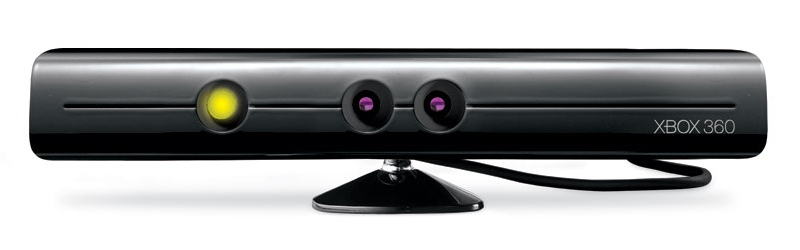
\includegraphics[scale=0.2]{img/kinect.jpg}
    \caption{Kinect - Dispositif utilisé pour la capture des images}
  \end{center}
\end{figure}

\subsection{L'environnement de travail}

Le projet est développé sous un système d'exploitation linux, en
utilisant un système de contrôle de version git
(https://github.com/tiagochst/PIM2013).  
De plus, les librairies externes utilisés sont:

\begin{description}

\item[Eigen] Une bibliothèque que met en oeuvre l'algèbre linéaire et des opérations matricielles.\cite{Eigen}

\item[OpenNI] Un framework qui fournit un ensemble d'API open source
  pour accéder aux périphériques d'interactions naturelles.\cite{PrimeSense2010}

\item[QT] Un framework qui fournit un ensemble d'API open source
  pour la création des interfaces.\cite{QT}

\item[OpenMP] Une interface de programmation pour le calcul parallèle
  sur architecture à mémoire partagée.\cite{OpenMP} 

\end{description}

Pour la compilation du projet nous l’outil qmake
pour une génération des Makefiles pour faciles et aussi intégré avec
le framework qt.  
Pour cela les fichiers suivants ont été crées: PIM380.pro. 

Par ailleurs, pour avoir un suivi plus visuel de l’état du projet on
utilise un outil en ligne pour la création d’un
kanban(http://kanbanize.com/) dont l’objectif est d’afficher la
situation actuel du projet. Ainsi, le kanban peut vous montrer ce qui
est en train d’être fait, ce qui a été fait, ce qui doit être fait,
les tests à faire et les bugs à traiter qui ont été trouvés. 

Finalement, pour la création de la documentation du code du projet, le
logiciel doxygen a été utilisé.  


\subsection{Méthodes}

Basée sur la méthode réalisé dans le papier ``High-quality passive
facial performance capture using anchor
frame''\cite{Beeler:2011:HPF:2010324.1964970} pour la reproduction
d'une reconstruction 3D de visages, on a divisé le projet en cinq
étapes listé ci-dessous: 

\begin{enumerate}
\item Calcul du maillage initial
\item Ancrage
\item Localisation image-space
\item Propagation de la maillage
\item Raffinement de maillage
\end{enumerate}

Ci-dessous une bref descrition de chaque étape:

\subsubsection*{Etape 1: Calcul du maillage initial}
Chaque image de la séquence est traitée indépendamment pour générer
une première estimation de la maillage pour cette trame. 

\subsubsection*{Etape 2: Ancrage}
Une trame est identifié manuellemnt comme la trame de réference. Puis,
les trames qui ont une apparance similaire (expression du visage
samblable et l'orientation de la tête) sont identifiées
automatiquement et étiquetés comme des trames d'ancrage. Ces trames
ancres seront un moyen de partitionner la séquence complète des clips
de trames pour le traitement dans la prochaine étape. 

\subsubsection*{Etape 3: Localisation image-space}
Le but de cette étape est de suivre les pixels de l'image à partir du
trame de référence pour chaque image dans la séquence.  

Le processus commence par le suivi de pixels d'image à partir de la
trame de référence pour les trames d'ancrage, ce qui est simple, car
l'aspect de l'image en deux trames est, par définition,
similaire. Cela permettra d'orienter le cheminement de pixels d'image
à partir de la trame de référence à toutes les autres trames dans la
séquence.  
Le suivi des trames non ancres est réalisé de manière séquentielle, à
partir des trames ancres les plus proches.

\subsubsection*{Etape 4: Propagation de la maillage}

Une propagation de maille désigne le calcul de nouvelles positions des
sommets du maillage dans l'espace, en correspondance avec le mouvement
physique de la face.

Un moyen pour propager la la maillage de référence (maillage de la
trame de référence calculé à l'étape 1, pour toutes les trames dans
la séquence, est l'utilisation des pixels de l'image suivis obtenues à
l'étape 3.
 
\subsubsection*{Etape 5: Raffinement de maillage}

Les étapes précédentes ont généré une propagation de la maille de
référence pour chaque trame dans la séquence. Cette séquence de
maillage déformant fournit une estimation initiale du mouvement du
visage, ce qui est raffiné pour garantir la cohérence avec les données
d'image en appliquant priori sur la cohérence spatiale et temporelle
de la surface déformée.

Le diagramme ci-dessous, présent plus visuallement les étapes du projet.

\begin{figure}[ht!]
  \begin{center}
    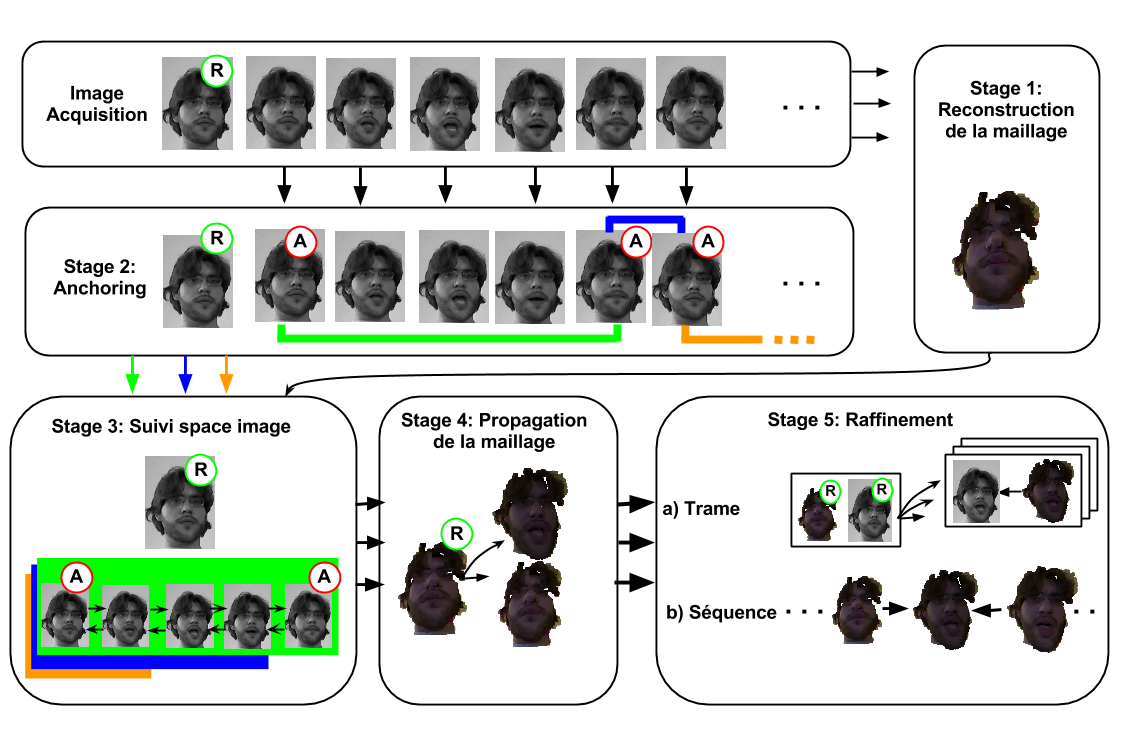
\includegraphics[scale=0.4]{img/projDiagram.png}
    \caption{Etapes du projet}
  \end{center}
\end{figure}




\newpage
\section{Les étapes de développement}
\subsection*{Interface Kinect}

Un des objectives du projet est d’avoir une interface avec la Kinect
pour capturer les images nécessaires pour la reconstruction faciale.

Pour qu’on puisse accéder aux données du dispositif Kinect, l’API
OpenNI\cite{Openni2010} a été utilisé. Cette API fournit des
interfaces de communication qui interagissent à la fois avec les
capteurs et les composants intermédiaires, qui analysent les données
provenant des capteurs.

\begin{figure}[h!]
  \begin{center}
    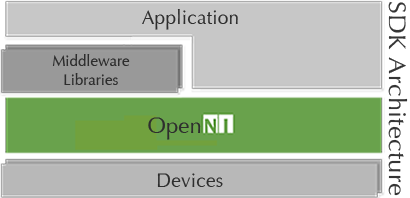
\includegraphics[scale=0.4]{img/image03.png}
    \caption{Architecture Openni}
  \end{center}
\end{figure}


La Kinect nous fournit une image RGB et sa profondeur en niveaux de
gris dans une résolution VGA (640×480).

Actuellement, quand la fonction de la caméra est appelée, on accédera
aux données de la Kinect et on dessinera par défaut la carte de
profondeur par dessus de la carte graphique. 

%Pour une interaction, les actions suivantes sont possibles: 

% tabela

La sortie peut être vue ci-dessous:

\begin{center} 
  \begin{figure}
    \centering
      \begin{subfigure}[b]{0.3\textwidth}
      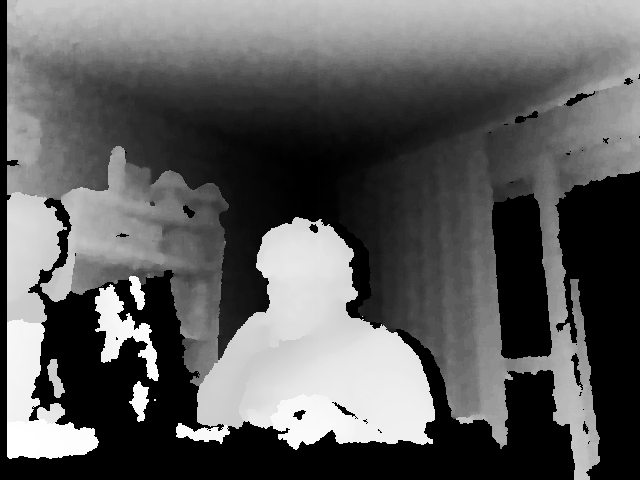
\includegraphics[scale=0.25]{img/image00}
      \caption{Carte de profundeur}
      \label{fig:cartedeprofondeur}
      \end{subfigure}%
      ~
      \begin{subfigure}[b]{0.3\textwidth}
        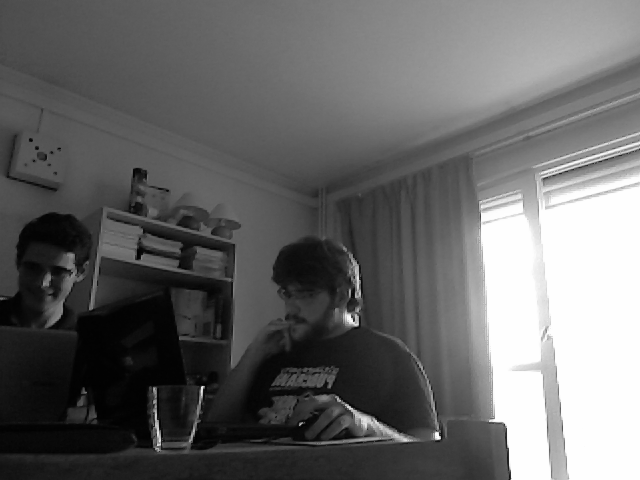
\includegraphics[scale=0.25]{img/image09}
      \caption{Sortie de la Kinect}
      \label{fig:kinectsortie}
      \end{subfigure}%
  \end{figure}
\end{center}


\subsection*{Interface graphique}

Pour une intéraction plus facile avec les utilisateurs, nous avons
décidé de créer une interface graphique. Le processus pour la création
a passé pour une identification des functionalitées qui était utiles
pour l'utilisateur. Quelques fonctionalité sont listées ci-dessous:

\begin{itemize}
\item Visualisation de l'entré de la Kinect 
\item Exportation de la maille affiché
\item Sauvegarder une séquence des trames
\item Séléction automatique des trames ancres
\item Edition manuel des trames ancres
\item Controler les paramètres principaux du programe
\item Calculer la carte de déplacement entre deux images
\end{itemize}

Après la phase d'indentification des fonctionalités, des idées on été
dessinées dans l'outil pencil\cite{Pencil}, un outil pour faire la
maquette de l'interface. 
Ci-dessous, la maquette pour la séléction automatique des trames ancres.

\begin{figure}[h!]
  \begin{center}
    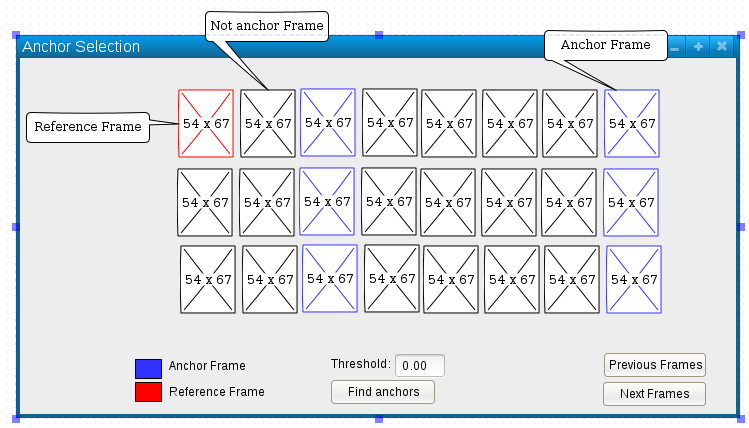
\includegraphics[scale=0.4]{img/pencil.png}
    \caption{Maquete: selection automatique de trames ancres}
  \end{center}
\end{figure}


Puis, l'interface graphique pour la visualisation des images et des
objets 3D a été crée en utilisant le framework QT et la librairie
QGLviewer. 
Pour la sélection des  frames ancres on a deux interfaces, une pour la
sélection manuel et l’autre pour la sélection automatique. Les images
de l’interface sont ci-dessous:

\newpage
Sélection d'ancres manuellement: 

\begin{figure}[ht!]
  \begin{center}
    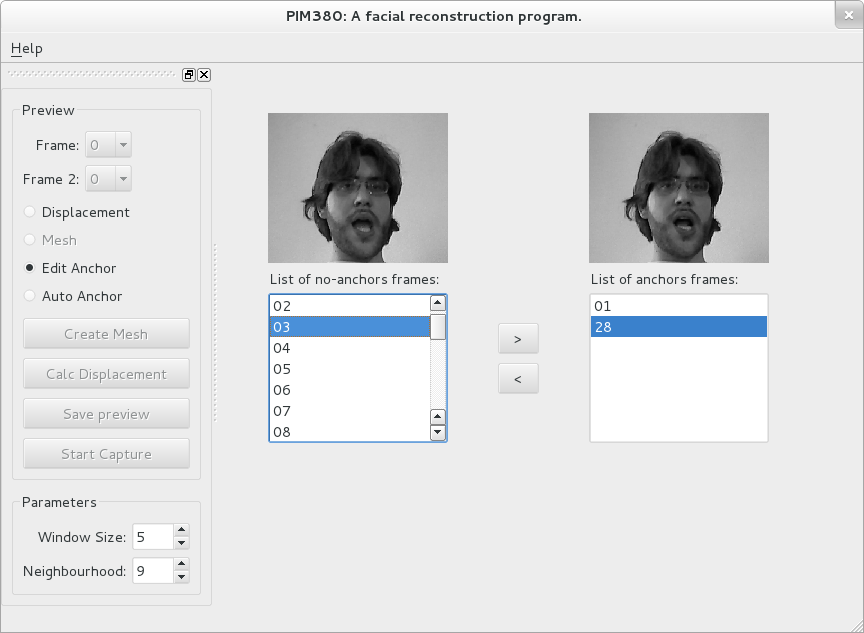
\includegraphics[scale=0.35]{img/editAnchorList.png}
    \caption{Edition de la liste des ancres}
  \end{center}
\end{figure}

Sélection d'ancres automatiquement:

\begin{figure}[ht!]
  \begin{center}
    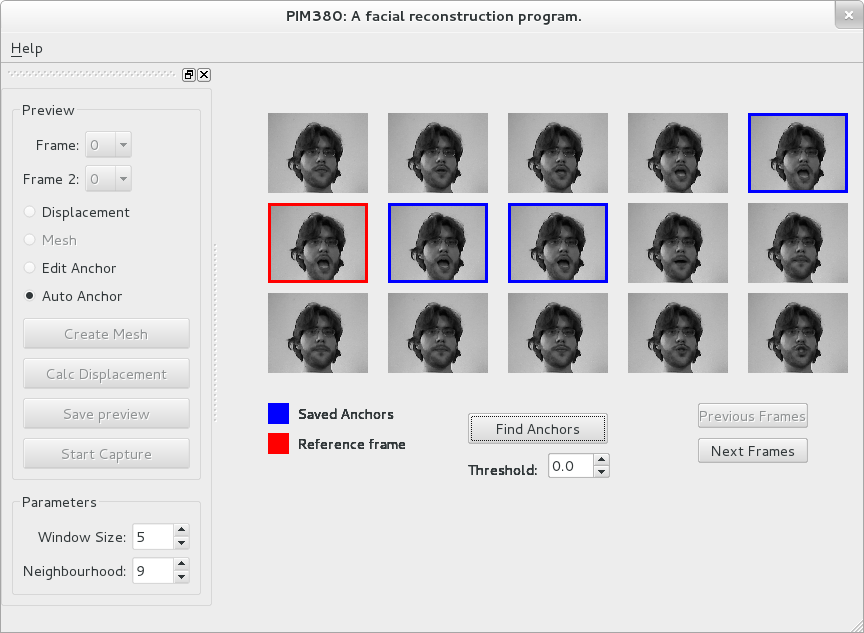
\includegraphics[scale=0.35]{img/AnchorAutomaticSelection.png}
    \caption{Séléction automatique des ancres. Entrée: trame de référence (rouge) et seuil. Sortie: trames ancres (bleau)}
  \end{center}
\end{figure}

\newpage
\subsection{Correspondance des pixels}

Pour la correspondance des pixels entre deux images, on évalue utilise
un algorithme basée sur la valuer de la intercorrélation normalisée
calculée sur une fenêtre carrée (3x3). La valeur la plus haute est
notre meilleur correspondance. 

D'abord, le Pixel $p$ dans l'image $I$ est comparé à tous les pixels
dans l'image $J$ dans une zone de recherche donné, et la meilleure
correspondance est conservée.  

Après avoir la meilleur correspondance, l'écart au pixel $p$ est
calculé en utilisant les valeurs de la intercorrélation normalisée
avec le point $p$ et ses deux voisins dans l'image $J$. En utilisant
ses trois points, on utilisé un polynôme de degré deux pour trouver la
valeur maximun que sera la valeur de la disparité. 

Pour l'utilisation des piramides des images, la correspondance est
calculée pour tous les pixels en utilisant les estimations de la
disparité de la couche précédente pour limiter la zone de recherche.  

En suite, pour certifier la bonne correspondance entre les pixels,
quelques constraintes on été implementées, pour validé la
correpondance.
\begin{description}

\item[Lissage] Pour avoir une cohérence entre les voisins, plus de la
  moitié de tous les voisins dans une fenêtre 3 x 3 diffèrent par un
  écart de moins d'un pixel de la disparité calculée au pixel $p$.  

\item[Unicité] la corresponce doit être bijective, c'est-à-dire si le
  pixel $p$ dans l'image $I$ correspond au pixel $q$ dans l'image $J$,
  alors $q$ doit également correspondre à $p$. Pour cette constrainte
  une disparité d'un pixel est acceptè.
\item[Ordre] Disparité calculée au point $p$ ne dépasse pas la
  disparité de son pixel droit voisin par plus d'un pixel.
\end{description}

Pour les pixels qui ne remplissent pas ces contraintes, la
correspondance sera rafait, mais cette fois, les estimations de la
disparité des pixels voisins qui on remplit les contraintes seront
utilisées. 

\begin{figure}[ht!]
  \begin{center}
    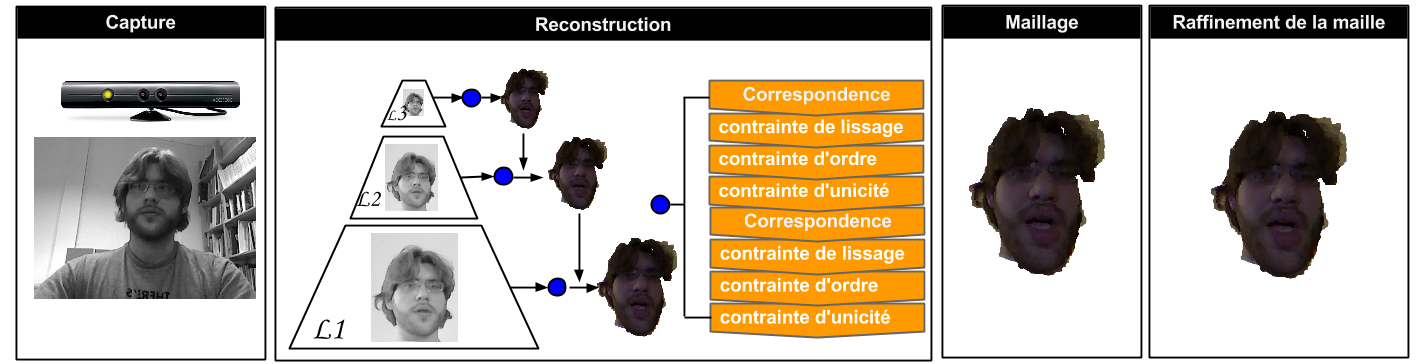
\includegraphics[scale=0.35]{img/projSystem.png}
    \caption{Le système proposé: de la capture à la reconstruction finale}
  \end{center}
\end{figure}

Le resultat de cette étape, est un map de disparité, contenant pour
chaque pixel de l'image $I$, la valeur de displacement dans l'image
$J$. 

\begin{figure}[ht!]
  \begin{center}
    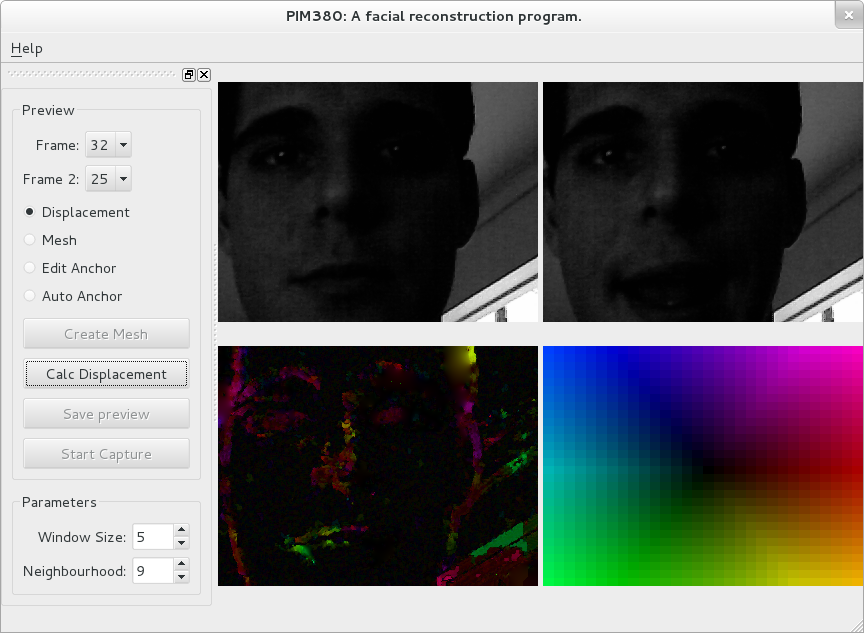
\includegraphics[scale=0.4]{img/dispMap.png}
    \caption{Sortie: Carte de déplacement}
  \end{center}
\end{figure}


\newpage
\subsection{Raffinement}

Le processus de raffinement est réalisé à deux étages, le premier est le
raffinement de la carte de disparité et la deuxième est le raffinement
de la surface.  

Le raffinement consiste en une combinaison linéaire de deux termes: un
terme cohérence photométrique $d_p$ qui privilégie les solutions à
haute intercorrélation normalisée et un terme de consistance de
surface $d_s$ qui privilégie les solutions lisses.

Ces termes sont équilibrées à la fois par un paramètre lissage
spécifié par l'utilisateur $w_s$ et un paramètre $w_p$ définit en temps
d'éxecution qui garantit que le terme photométrique a plus de poids
dans les régions avec une bonne fonctionnalité de localisation.

Les étapes pour les calculs de ces termes sont:
\begin{enumerate}
\item Compute $d_p$:

\begin{eqnarray*}
u_{p}=\begin{cases}
p - q - 0.5 & \xi_{-1}<\xi_{0},\xi_{+1}\\
p - q + 0.5\frac{(\xi_{-1}-\xi_{-1})}{\xi_{-1}+\xi_{+1}-2\xi_{0}} &
\xi_{0}<\xi_{-1},\xi_{+1}\\ 
p - q + 0.5 & \xi_{+1}<\xi_{0},\xi_{-1}
\end{cases}
\end{eqnarray*}

\item Compute $w_p$:
\begin{eqnarray*}
w_{p}=\begin{cases}
\xi_{0}-\xi_{-1} & \xi_{-1}<\xi_{0},\xi_{+1}\\
0.5(\xi_{-1}+\xi_{+1}-2\xi_{0}) & \xi_{0}<\xi_{-1},\xi_{+1}\\
\xi_{0}-\xi_{+1} & \xi_{+1}<\xi_{0},\xi_{-1}
\end{cases}
\end{eqnarray*}

\item Compute $u_s$:

\[
u_{s}(x,y)=\sum_{(x^{'}y^{'})\epsilon\aleph(x,y)}w_{x^{'},y^{'}}u_{x^{',y^{'}}}\frac{1}{\sum_{(x^{'}y^{'})\epsilon\aleph(x,y)}} 
\]

Où:$w_{x^{'},y^{'}}:=exp\left(\frac{\parallel\delta_{x^{'}y^{'}}-\delta_{xy}\parallel}{\sigma^{2}}\right)(1-\xi_{x^{'}y^{'}})$
et $\aleph$ désigne le pixel plus la voisinage de (x, y), les 8 pixels
voisins. De plus, $\epsilon$ est $1mm$ selon notre matériel de capture
(précision de la kinect). 

\item Compute $d^{'}$, la nouvelle valeur de disparité pour le pixel $p$:
$d^{'}=\frac{(w_{p}u_{p}+w_{s}u_{s})}{(w_{p}+w_{s})}$

Où la valeur de $w_{s}$ dans notre programme vaut $0.005$.

\end{enumerate}

\newpage
\section{Résultats}

La figure ci-dessous (figure \ref{fig:trames910}) présent notre
dernière trame d'une séquence pendant laquelle notre acteur ouvre la bouche. 

\begin{figure}[ht!]
        \centering
        \begin{subfigure}[b]{0.5\textwidth}
                \centering
                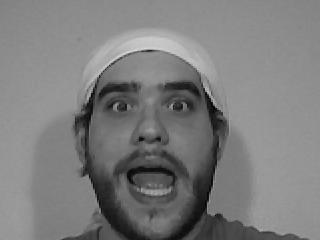
\includegraphics[width=\textwidth]{img/f9}
                \caption{Trame 9}
                \label{fig:trame9}
        \end{subfigure}%
        ~ %add desired spacing between images, e. g. ~, \quad, \qquad etc.
          %(or a blank line to force the subfigure onto a new line)
        \begin{subfigure}[b]{0.5\textwidth}
                \centering
                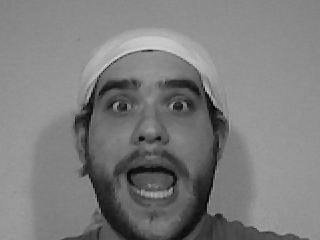
\includegraphics[width=\textwidth]{img/f10}
                \caption{Trame 10}
                \label{fig:trame10}
        \end{subfigure}
        \caption{Séquence d'ouverture de la bouche}
        \label{fig:trames910}
\end{figure}

Nous pouvons vérifier en utilisant la carte de couleur de déplacement
(figure \ref{fig:colorChart}), que la région de la buche a une valeur
vert ce qui répresent un déplacement vers le bas.

\begin{figure}[h!]
  \begin{center}
    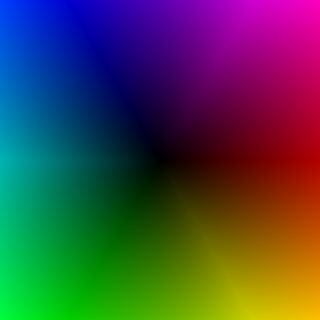
\includegraphics[scale=0.6]{img/ColorChart}
    \caption{Valeurs de déplacement répresentés par les coulers}
    \label{fig:colorChart}
  \end{center}
\end{figure}

Nous pouvons vérifier en utilisant la carte de couleur de déplacement
(figure \ref{fig:colorChart}), que la région de la buche a une valeur
vert ce qui répresent un déplacement vers le bas.

Après le calcul de déplacement entre les trames, on commence a
propager les sommets de la maillage de référence en utilisant les
cartes de déplacements calculés. Notre résultat, est affiché dans
l'image ci-dessous (figure \ref{fig:result}). La figure en haute à
gauche est notre maillage de réference propagé jusqu'au trame 10.

% 37
% 250
% 305
 
\begin{figure}[ht!]
  \begin{center}
    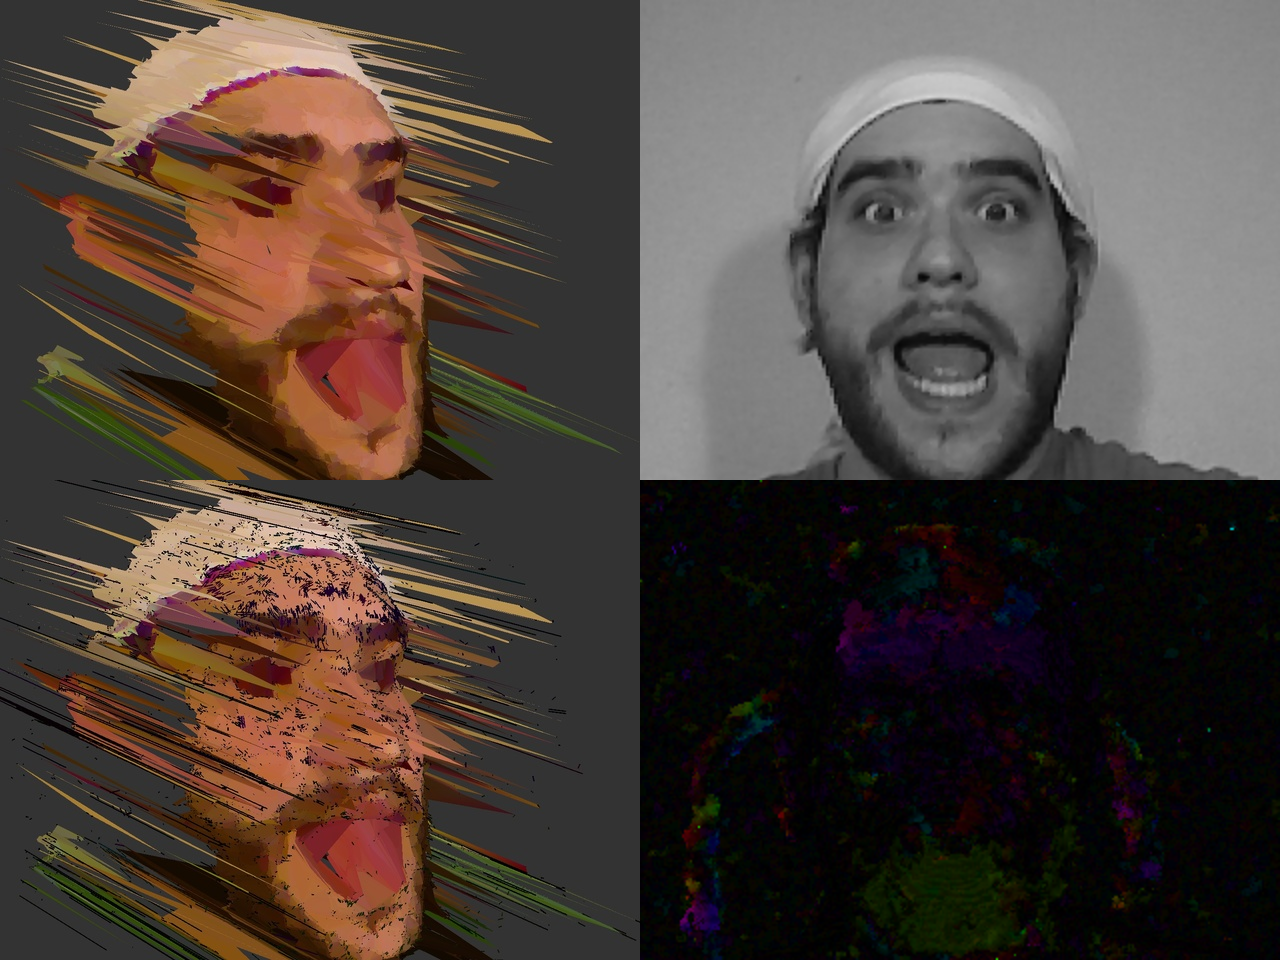
\includegraphics[scale=0.4]{img/frame10}
    \caption{Résultats: haute gauche: maillage propragée,haute droite:
      trame actuelle, bas gauche: maillage avec les déplacement em 3D,
      bash droite: carte de déplacement }
    \label{fig:result}
  \end{center}
\end{figure}

\section{Conclusion}

%Nous avons implementé dans ce projet une méthode de capture 
%passive qui emploi deux tecnhiques clées baseés sur l'article de Beeler et
%al. \cite{Beeler:2011:HPF:2010324.1964970,}.

%Tout d'abord, nous employons un algorithme de corresponsance qui intègre
%toutes les correspondence de pixels dans l'espace image, le résultat
%de cette étape est intégré pour propager une seule maille de référence pour chaque trame cible en parallèle. 
% 
%Deuxièmement, comme les performances du visage ont tendance à contenir
%les mouvements répétitifs, l'idée des «trames d'ancrage»
%définis comme ceux dont l'expression du visage est semblable au cadre de référence.
% 
%Après localisation automatique des trames d'ancrage, on calcule le
%suivi des pixels directement à partir de la trame de référence à des
%trames d'ancrage. En utilisant les trames d'ancrage à la partition de
%la séquence dans les clips et l'appariement indépendamment clips, nous
%sommes en mesure de dérive tracker lié, gérer correctement occlusion
%et le flou de mouvement, et des séquences de capture de processus en parallèle. 

%Notre méthode produit une géométrie 3D détaillées en correspondance
%temporelle complète, même pour le plus expressif des performances en
%cours de mouvement très rapide, sans qu'il soit nécessaire de
%marqueurs placés à la main ou le maquillage du visage. 
%Nous avons démontré notre technique sur un certain nombre d'exemples de
%représentations données par les différents acteurs, et nous avons
%également montré comment notre approche ancrée de reconstruction
%combiné avec notre méthode de tracking image-espace robuste peut
%donner des résultats plus précis qu'un-of-the-art de l'État actuel
%technique [Bradley et al. 2010], en particulier en présence de motion
%blur et les rides très expressives où dérive a tendance à s'accumuler
%plus rapidement.

La qualité du équipement de capture a eu une grand influence sur notre
résultat. Téoriquement la précision de la Kinect pour les valuers de
profondeurs est de 1mm, par contre, nous avons aperçu dans nos
premières résultat que, pour les points plus loins, cette
précision n'est pas valable, car la kinect produissait une sortie avec
des erreurs bien plus grands que $10 mm$. 
En raison de ce problème, nous avons dévélopper notre algorithme de
manière a minimizer ce problème.

De plus, pour quelques points la kinect ne reconnait pas la
profondeur, ce qui a introduit un problème en plus pour l'algorithme. 
Pour contourne ce problème, nous avons fixer ces valerus inconnues à
0. 

Une autre question lié à la kinect qui influencie nos résultats et
implémentation sont les images dont la résolution est 13 fois plus
petite que celles de l'article, ainsi, en raison de notre situation
quelques paramètres on été adaptées.

A titre d'exemple, pour la sélection automatique des trames, l'article
prennait un pixel sur 20 pour faire une comparaison de similarité
entre deux images. Pour une image $1176 x 864$ pixels, cela nous donne
environ $50803$ pixels. Dans notre cas por une image $320 \times 240$ pixels,
cela nous donne seulement $3840$ pixels. C'est-à-dire, moins que 10\% du
nombre de pixels utilisé dans article. Pour résoudré cela, on a pris 1
pixel sur 3, ce qui nous donne environ $25600$ pixels un nombre de
pixels plus acceptable.

Une autre modification lié à la résolution des images, est
l'utilisation d'un patch de $17 \times 17$ au lieu d'utiliser un patch
$9 \times 9$ pour faire le calcul de similarité à travers de la
intercorrélation normalisée. Cela nous a aporté une réponse plus
fiable de la similarité.   


\section{Remerciement}
Nous tiendrons tout d’abord à remercier Dr Tamy Boubekeur, le
professeur responsable du projet et notre tuteur, de nous avoir
accueilli comme élévés au sein du projet et la confiance qu’il nous a
accordé tout au long de notre projet. 

Nous remercions également Thierry Guillemot et Stéphane Calderon, pour
leur volonté à nous aider pendant toute la période de notre projet PIM. 

\nocite{Beeler:2010:HSC:1778765.1778777}

% ******************************************************
% REFERENCIAS BIBLIOGRÁFICAS
% ******************************************************
\begin{small}
  \bibliography{pim}
\end{small}
\section*{}

\end{document}
